\documentclass[conference]{IEEEtran}
\IEEEoverridecommandlockouts

% Packages
\usepackage{cite}
\usepackage{subcaption}
\usepackage{amsmath,amsfonts}
\usepackage{algorithm}
\usepackage{algpseudocode}
\usepackage{graphicx}
\usepackage{textcomp}
\usepackage{xcolor}
\usepackage{booktabs}
\usepackage{adjustbox}
\usepackage{listings}
\usepackage{hyperref}
\usepackage{verbatim}
\usepackage{multirow}
\usepackage{placeins}
\usepackage{subcaption}

\newcommand{\todo}[1]{\color{red} TODO #1\color{black}}
\newcommand{\torem}[1]{\color{olive} #1 \color{black}}


\def\BibTeX{{\rm B\kern-.05em{\sc i\kern-.025em b}\kern-.08em
    T\kern-.1667em\lower.7ex\hbox{E}\kern-.125emX}}



\begin{document}

\title{Second Deliverable report \\
\footnotesize \textit{"Matteo Di Noia": Mat: 258426, \texttt{matteo.dinoia@unitn.it}, GitRepo: \texttt{\href{https://github.com/matteo-dinoia/GPU-Computing-2025-258426}{matteo.dinoia/GPU-Computing-2025-258426}}}}

\maketitle

\begin{abstract}
%\torem{[max 200 words]}\\
The sparse matrix-dense vector multiplication (SpMV) is a common linear algebra operation consisting of a matrix multiplication between, as the name implies, a sparse matrix and a dense vector. SpMV is widely used in many real-world applications such as scientific computing and graph analytics.

This paper covers one of the possible representation used for sparse matrix in SpMV, COO. Of this problem, this paper quickly discuss CPU implementation and then focuses on GPU implementation, both naive version and more advanced versions using prefix sum, shared memory and warp operation. To do so we will need to add some sorting assumption to COO. Finally, the various results are compared and are suggested combination of the best kernels with some heuristic.
\end{abstract}

\begin{IEEEkeywords}
Sparse Matrix, SpMV, CUDA, Parallelization, Storage Format, Prefix Sum
\end{IEEEkeywords}

\section{Introduction}
%\torem{[max 300 words]Introduce SpMV application and its parallelization challenges \dots}\\

Sparse matrix vector multiplication (SpMV) is a core computation that is at the foundation of every implicit sparse linear algebra solver. It is also one of the most common primitive in scientific computing, and graph analytics, eg. it is present in software such as MatLab and Numpy.

Due to being an intrinsically memory-bound algorithm, its performance are limited by the bandwidth between the process and the memory, especially on highly parallelized, throughput-oriented architectures such as GPU.


\section{Problem Statement}
%\torem{Define the problem statement, including a description of the storage format used and a brief discussion of the parallelization approach (e.g., using CUDA).}
Sparse matrix vector multiplication (SpMV) is a matrix multiplication between a matrix $A$ of size $n\times m$ and a vector $x$ of size $m\times 1$, which result in a vector $y$ of size $n\times 1$ computed as follows:

\[y=A \cdot x\]
\[y_i = \sum_{k=1}^{n}A_{ik} x_{k}\]

\begin{figure}[h!]
	\centering
	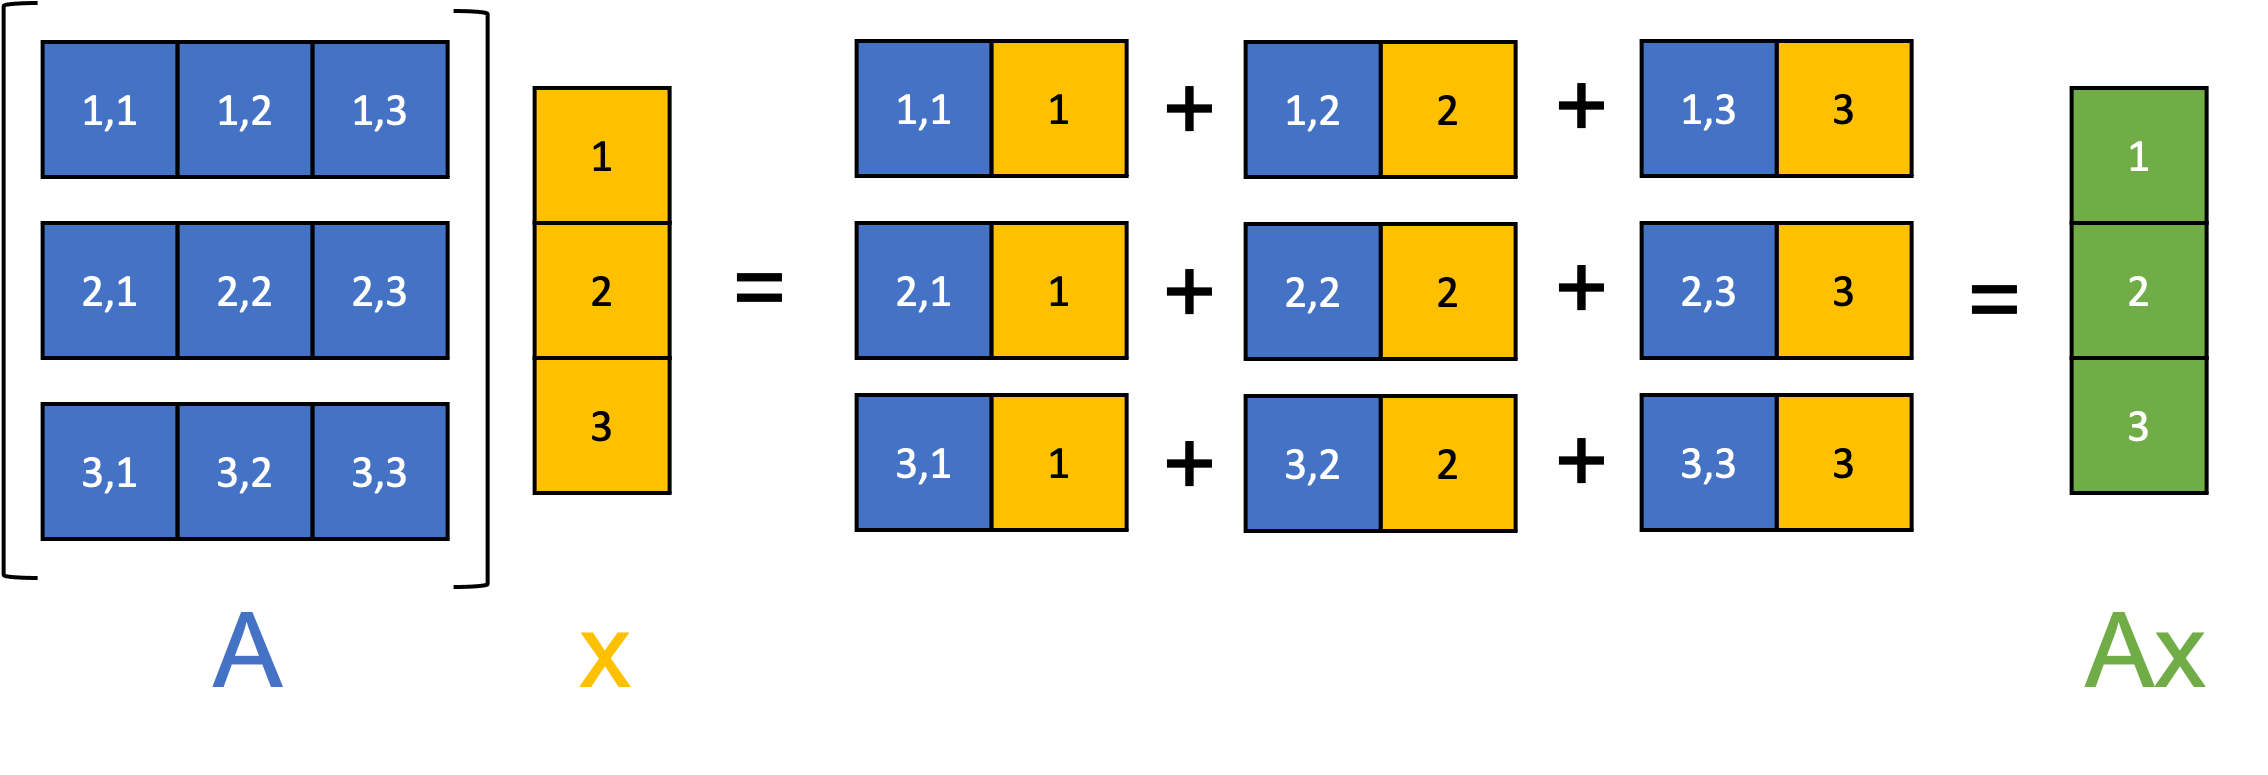
\includegraphics[width=0.9\linewidth]{other_img/matrix_vec_mult}
	\caption{Matrix Vector Multiplication}
	\label{fig:matrixvecmult}
\end{figure}
%TODO reference https://mbernste.github.io/posts/matrix_vector_mult/

The particularity of Spmv, is that the matrix is sparse, meaning that most of its elements are empty (contains zero) and while the vector is dense, as in not sparse.



An efficient implementation of SpMV present various challenges, most of which are related to choosing a good storage format and having an efficient memory access. The latter of which, is required because, as mentioned before, SpMV is a memory-bound algorithm. In fact the arithmetic intensity, meaning the worst-case ratio between the number of arithmetic operation over the number of read/write operation , is very low:
\[Intensity = \frac{2\ flop}{6 \cdot 4\ bytes} = 0.083\frac {flop}{bytes}\]
Instead the role of the storage format, during the program execution, is to facilitate such access.

\subsection{Storage Format}
%\torem{Details about the format (e.g., CSR, COO, etc.) \dots}

Multiple format exists such as Compressed Sparse Row (CSR), Coordinate (COO), ELLPACK (ELL), etc. In the present paper, the analysis is concentrated over the COO format. The latter is the simplest one, in which three array are used to represent the matrix:

\begin{figure}[h!]
	\centering
	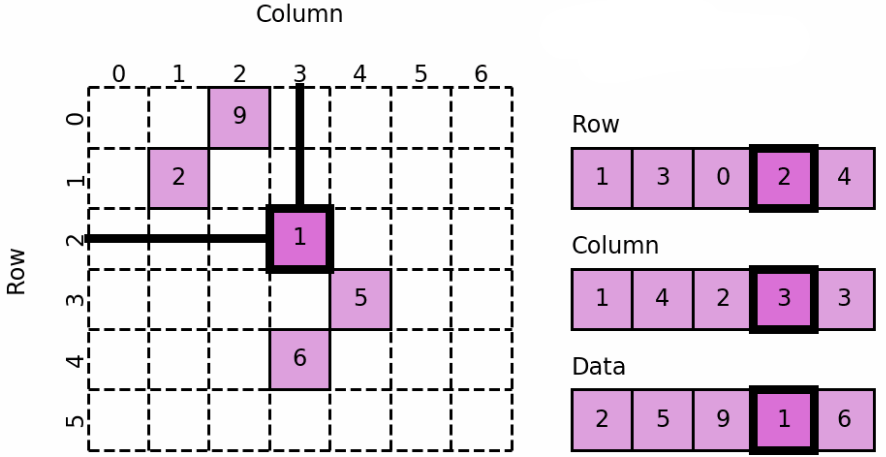
\includegraphics[width=0.9\linewidth]{other_img/coo}
	\caption{Example of COO format}
	\label{fig:coo}
\end{figure}
% TODO reference https://firas-jolha.github.io/bigdata2025/html/bs/BS%20-%20Lab%208%20-%20Apache%20Spark%20MLlib.html

\begin{itemize}
	\item \textbf{rows (/Ys)}: containing for every $i$ the row (or $y$ value), in which the $i$-th element of the matrix is;
	\item \textbf{cols (/Xs)}: containing for every $i$ the column (or $x$ value), in which the $i$-th element of the matrix is
	\item \textbf{values (/data)}: containing for every $i$ the value of $i$-th element;
\end{itemize}

While the COO format may have no sorting guarantees, during the analysis of this paper it will be assumed the use of a COO sorted by row index and then by column index. This is required as the optimized kernel using prefix-sum are based on that assumption.
\[el1 < el2 := row1 < row2 \lor (row1 = row2 \land col1 < col2) \]

This make the format, partially, similar to Compressed Row Format (CSR); with the difference that in CSR the row vector is compressed, as the name implies, to an array contains pointers that mark the beginning of rows within the column and value array. CSR format will also be mentioned as point of comparison of the CPU implementation.

\begin{figure}[h!]
	\centering
	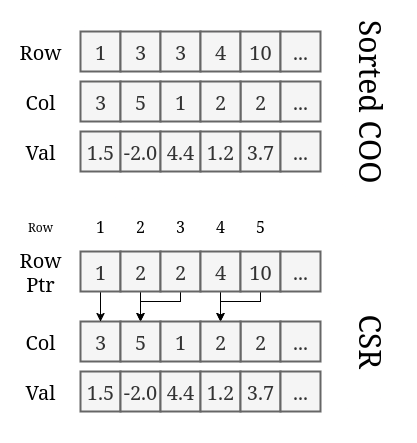
\includegraphics[width=0.7\linewidth]{other_img/diagram-csr-sorted-coo}
	\caption{Sorted COO and CSR format}
	\label{fig:diagram-csr-sorted-coo}
\end{figure}


\subsection{Parallelization}
%Describe the CUDA implementation approach \dots
Being SpMV a conceptually easy operation, in order to parallelize it we can exploit independence between operation on some blocks of data, to obtain data parallelism.

The simplest way to split the data and to parallelize the operation, is to have a thread for each element in the COO format. This is simple but while the read operation on the matrix and the multiplying vector are not interfering; the write, in particular it is a read followed by an addition and finally a write, to the result vector can happen at the same time another thread is doing the same time it is accessing the same location. This is a race condition and to avoid it, atomic operations are required. The operation in question needed is $atomicAdd$, which perform read, addition and write atomically.

\begin{figure}[h!]
	\centering
	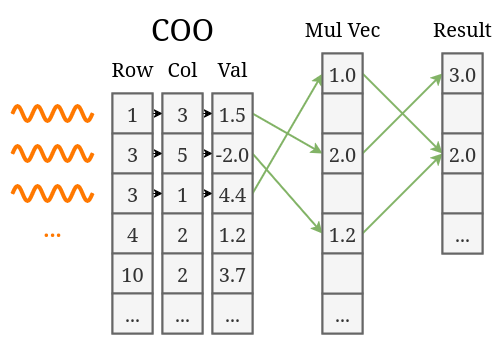
\includegraphics[width=0.7\linewidth]{other_img/diagram-threads}
	\caption{Simple parallelization idea and its faults}
	\label{fig:diagram-threads}
\end{figure}


But this approach has some limitations: the small but existing overhead of the atomic operation; but mostly the great amount of writing to same cell in the result vector. We can tackle the second one by exploiting the fact that to compute the product of a row and the vector it is only needed read access to the previous two and write access to a single element of the result vector.
\begin{figure}[h!]
	\centering
	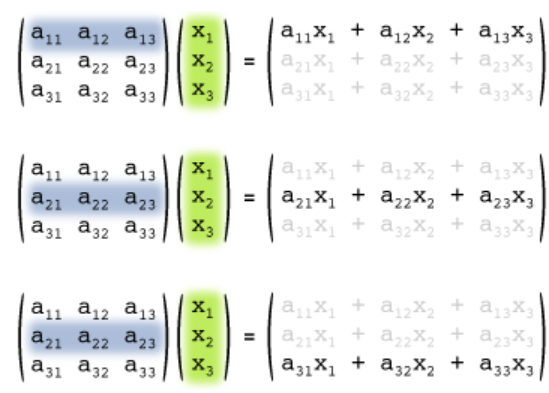
\includegraphics[width=0.7\linewidth]{other_img/row-independence}
	\caption{Eg. rows independence of matrix vector multiplication  }
	\label{fig:row-independence}
\end{figure}

Because of this we can have a single write for each row, possibly decreasing the amount of write if there are more than a single entry for row. But the major improvement of this method is that we reduce the number of time we write on the same location, which improve performance, especially when using $AtomicAdd$, because when multiple write are performed only one can succeed while the other need to wait.

\section{State of the Art}
The state of art SpMV for CPU is OpenBLAS, which is an optimized BLAS (Basic Linear Algebra Subprograms). On the other hand, cuSPARSE is a Cuda based GPU accelerated BLAS which perform significantly faster than CPU only alternatives thanks to the higher degree of parallelization.

\section{Methodology and Contributions}\label{sec:methodology}

%describe the methodology used during the analysis, the compared algorithms and the expected outcomes. Use pseudo-codes like Algorithm \ref{alg:COOaggr} to describe your own implemented kernels.

%\noindent Include at least the following implementations:
%\begin{itemize}
%    \item Naive CPU implementation
%    \item Optimised CPU implementation based on cache behaviour
%    \item GPU naive implementation
%\end{itemize}

For the analysis, a COO CPU \ref{alg:COO_CPU} and  naive GPU \ref{alg:COO_GPU} implementations were created. Both access data in the sparse matrix $A$ sequentially and the resulting vector $Y$ sequentially, sacrificing instead the sequentiality in the access of the dense multiplying vector $v$.

\begin{algorithm}[h!]
	\caption{COO SpMV on CPU}
	\algorithmicrequire~The input vectors $Ar$, $Ay$, $Av$ representing the COO matrix of size $nnz$, the vector $X$ of size $nrows$.
	\begin{algorithmic}[1]
		\Procedure{Function}{$Ar$, $Ay$, $Av$, $X$, $nnz$}
		\For{$k$ in $\{1 \dots nnz\}$}
		\State $Y[Ay[k]] = Y[Ay[k]] + Av[k] * X[Ax[k]] $\label{partitioning}
		\EndFor
		\State \textbf{return} $Y$\Comment{the result vector}
		\EndProcedure
	\end{algorithmic}
	\label{alg:COO_CPU}
\end{algorithm}

We also implemented a CSR CPU implementation to have a point of comparison for the CPU version. Because of the size difference between CSR and COO, with CSR being normally smaller because of the compressed rows array, we expect the throughput of the latter to be greater than the one of COO as both are memory-bound application.

\begin{algorithm}[h!]
	\caption{CSR SpMV on CPU}
	\algorithmicrequire~Same as before
	\begin{algorithmic}[1]

		\Procedure{Function}{$Ar$, $Acy$, $Av$, $X$, $nnz$, $nrows$}
		\State $k \leftarrow 0$
		\For{$r$ in $\{1 \dots nrows\}$}
		\State $end \leftarrow Acy[r + 1]$
		\While{$k < end$}
		\State $Y[r] \leftarrow Y[r] + Av[k] * X[Ax[k]] $\label{partitioning}
		\State $k \leftarrow k + 1$
		\EndWhile
		\EndFor
		\State \textbf{return} $Y$\Comment{the result vector}
		\EndProcedure
	\end{algorithmic}
	\label{alg:CSR_CPU}
\end{algorithm}
The simple CPU version \ref{alg:COO_CPU} can be parallelized, in order to make a baseline GPU version. This can be done by simply parallelizing the for, having a thread for each element of the matrix and replacing the assignment and addition with a $atomicAdd$, as shown in the following pseudo-code \ref{alg:COO_GPU} .

\begin{algorithm}[h!]
	\caption{GPU baseline COO SpMV}
	\algorithmicrequire~Same as before
	\begin{algorithmic}[1]
		\Procedure{Function}{$Ar$, $Ay$, $Av$, $X$, $nnz$}
		\For{$k$ in $\{1 \dots nnz\}\ \textbf{parallel}$}
		\State $atomicAdd(Y[Ay[k]],\ Av[k] * X[Ax[k]]) $\label{partitioning}
		\EndFor
		\State \textbf{return} $Y$\Comment{the result vector}
		\EndProcedure
	\end{algorithmic}
	\label{alg:COO_GPU}
\end{algorithm}

But this simplicity comes with a cost: performance. That is because this kernel does not tries to optimize memory access so that they are coalesced; also because each thread perform very little operation, most of the time is spent dispatching threads.

So the first thing, we tried implementing is different access pattern, with relation to which thread does which operation, allowing a single thread to run multiple to better make use of cache locality.


\begin{algorithm}[h!]
	\caption{Generic cache optimized GPU version}
	\algorithmicrequire~Same as before
	\begin{algorithmic}[1]
		\Procedure{Function}{$Ar$, $Ay$, $Av$, $X$, $nnz$}
		\For{$k$ in $\{1 \dots N\_THREADS\}\ \textbf{parallel}$}
		\State $per\_thread \leftarrow \text{ceil}(nnz / N\_THREADS)$
		\For{$j$ in $\{1 \dots per\_thread\}$}
		\State $el \leftarrow \text{custom\_map}(k, i)$
		\State $\text{atomicAdd}(Y[Ay[el]],\ Av[el] * X[Ax[el]]) $\label{partitioning}
		\EndFor
		\EndFor
		\State \textbf{return} $Y$\Comment{the result vector}
		\EndProcedure
	\end{algorithmic}
	\label{alg:GPU_cache_opt}
\end{algorithm}
\FloatBarrier

In this code the function $custom\_map$ is any map that make so that each entry in the COO format is visited one and only once; in the following chapter \ref{subsec:GPU}, we will compare various of this possible map with the baseline.


It is still possible to increase performance, especially in the case of multiple element per single row. That is because, as already mentioned, the previous code is writing multiple times to the same resulting vector. To reduce this write it is possible to compute the prefix sum of element and then for each row only adding the last element and remove the first prefix sum value for that row. That reduce the amount to a slightly more than 2 write for each row. Notice that the following code \ref{alg:prefix_sum_alg}, which compute the parallel prefix sum (also called scan), is partially incomplete for simplicity of explanation, avoiding handling size of COO not multiple of SIZE. SIZE is the unit of computation we can use synchronization primitive over it, in fact after every step of \ref{fig:naive-scan} it is required a `\_\_syncthread()` operation. Finally this is only partially a prefix sum, as it doesn't combine the result of multiple chunks of size SIZE because that would be more expensive than just doing two extra atomic add, at the end of the chunk (the start contains 0 so no operation is needed).



\begin{algorithm}[h!]
	\caption{Naive prefix sum algorithm}
	\algorithmicrequire~Same as before
	\begin{algorithmic}[1]
		\Procedure{Function}{$Ar$, $Ay$, $Av$, $X$, $nnz$}
		\For{$k$ in $\{1 \dots N\_THREADS\}\ \textbf{parallel}$}
			\State \Comment{Load elements to sum}
			\State $sum[k] \leftarrow  val[k] * vec[k]$
			\State{$el  \leftarrow  k ~\%~ SIZE$}
			\State \Comment{Compute prefix sum}
			\For{$s  \leftarrow  1;\ s < SIZE;\ s  \leftarrow  s / 2$}
				\If{$el + s < SIZE$}
					\State $sum[el + s]  \leftarrow sum[el + s] + sum[el]$
				\EndIf
			\EndFor
			\State \Comment{Save results to vector}

			\If{$el = SIZE - 1$}
				\State $\text{atomicAdd}(res[y[k]], sum[el])$
			\Else
				\If {$y[k] < y[k + 1]$}
					\State $\text{atomicAdd}(res[y[k]], sum[el])$
					\State $\text{atomicAdd}(res[y[k + 1]], -sum[el])$
				\EndIf
			\EndIf

		\EndFor
		\State \textbf{return} $Y$\Comment{the result vector}
		\EndProcedure
	\end{algorithmic}
	\label{alg:prefix_sum_alg}
\end{algorithm}

\begin{figure}[h!]
	\centering
	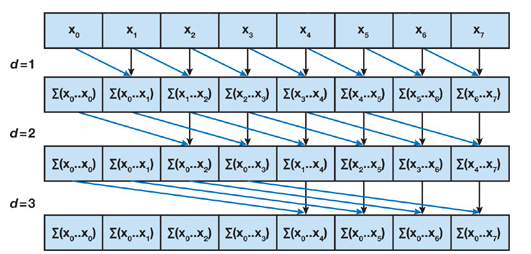
\includegraphics[width=0.9\linewidth]{other_img/naive-scan}
	\caption{Naive prefix-sum/scan}
	\label{fig:naive-scan}
\end{figure}
% TODO https://developer.nvidia.cn/gpugems/gpugems3/part-vi-gpu-computing/chapter-39-parallel-prefix-sum-scan-cuda
\FloatBarrier
Because it use about 2 write for each row, it is an improvement in most somewhat row dense matrix; but if most rows contain a single value, the previous algorithm would just instead compromise performance. To lower this number of write to almost a single write for row we need to do the prefix sum but only sum two elements if they are in the same row. In this case the last value of a row in the prefix sum is the value we searched and can add it to the result vector. Note in \ref{alg:prefix_sum_alg_equals} that the same problem with end of chunks remain.

\begin{algorithm}[h!]
	\caption{Naive prefix sum algorithm}
	\algorithmicrequire~Same as before
	\begin{algorithmic}[1]
		\Procedure{Function}{$Ar$, $Ay$, $Av$, $X$, $nnz$}
		\For{$k$ in $\{1 \dots N\_THREADS\}\ \textbf{parallel}$}
			\State \Comment{Load elements to sum}
			\State $sum[k] \leftarrow  val[k] * vec[k]$
			\State{$el  \leftarrow  k ~\%~ SIZE$}
			\State \Comment{Compute prefix sum}
			\For{$s  \leftarrow  1;\ s < SIZE;\ s  \leftarrow  s / 2$}
				\If{$el + s < SIZE$ \textbf{and} $y[el + s] = y[el]$}
					\State $sum[el + s]  \leftarrow sum[el + s] + sum[el]$
				\EndIf
			\EndFor
			\State \Comment{Save results to vector}
			\If{$el = SIZE - 1$ \textbf{or} $y[k] < y[k + 1]$}
				\State $\text{atomicAdd}(res[y[k]], sum[el])$
			\EndIf
		\EndFor
		\State \textbf{return} $Y$\Comment{the result vector}
		\EndProcedure
	\end{algorithmic}
	\label{alg:prefix_sum_alg_equals}
\end{algorithm}

Up to this point the thread cooperated with each other with the use of shared memory and synchronization primitive. But it is possible to compute the same code using warp primitive. A warp is a group of threads that are scheduled together and guaranteed to execute in parallel, and have some function that allow cooperation at the hardware level. The one we are interested in is `\_\_shfl\_up\_sync`, which share data from each thread in the thread to some thread n step on the right. In practice, in our use it perform a single step of figure \ref{fig:naive-scan}, over the size $WARP$ which is $WARP < SIZE$.

\begin{algorithm}[h!]
	\caption{Naive prefix sum algorithm}
	\algorithmicrequire~Same as before
	\begin{algorithmic}[1]
		\Procedure{Function}{$Ar$, $Ay$, $Av$, $X$, $nnz$}
		\For{$k$ in $\{1 \dots N\_THREADS\}\ \textbf{parallel}$}
		\State \Comment{Load elements to sum}
		\State $sum\_i \leftarrow  val[k] * vec[k]$
		\State $yi \leftarrow  y[k]$
		\State{$tid\_warp  \leftarrow  k ~\%~ WARP$}
		\State \Comment{Compute prefix sum}
		\For{$s  \leftarrow  1;\ s < SIZE;\ s  \leftarrow  s / 2$}
		\State {$to\_add = \text{\_\_shfl\_up\_sync}(sum\_i, s)$}
		\State {$yi2 = \text{\_\_shfl\_up\_sync}(yi, s)$}
		\If{$tid\_warp >= s$ \textbf{and} $yi2 = yi$}
		\State $sum\_i \leftarrow sum\_i + to\_add;$
		\EndIf
		\EndFor
		\State \Comment{Save results to vector}
		\State {$y\_next = \text{\_\_shfl\_down\_sync}(yi, 1)$}
		\If{$tid\_warp = WARP - 1$ \textbf{or} $yi < y\_next$}
		\State $\text{atomicAdd}(res[yi], sum\_i)$
		\EndIf
		\EndFor
		\State \textbf{return} $Y$\Comment{the result vector}
		\EndProcedure
	\end{algorithmic}
	\label{alg:prefix_sum_alg_equals}
\end{algorithm}
\FloatBarrier

In our case $WARP=32$ and $SIZE=1024=32^2$ so we can use other two prefix sum to have a prefix sum over a single chuck of size SIZE. The code is not here reported, but the idea of the procedure is represented in the figure
\begin{figure}[h!]
	\centering
	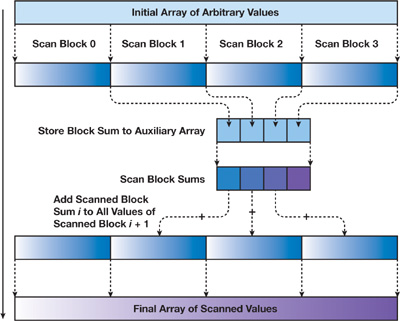
\includegraphics[width=0.8\linewidth]{other_img/complete-prefix}
	\caption{Prefix sum from WARP size to SIZE size}
	\label{fig:complete-prefix}
\end{figure}
%TODO http://developer.nvidia.cn/gpugems/gpugems3/part-vi-gpu-computing/chapter-39-parallel-prefix-sum-scan-cuda

Finally some other algorithms were tested to implement an efficient prefix sum, but the result were not much better in most cases, and as such are here and in the result chapter only cited, the code for the work efficient, bank-conflict free version in the  \href{http://developer.nvidia.cn/gpugems/gpugems3/part-vi-gpu-computing/chapter-39-parallel-prefix-sum-scan-cuda}{NVIDIA book}.
%TODO http://developer.nvidia.cn/gpugems/gpugems3/part-vi-gpu-computing/chapter-39-parallel-prefix-sum-scan-cuda

\section{System Description and Experimental Set-up}
%Use this section to describe system, dataset and experimental set-up.

\subsection{System Description}
%Describe the used system and the software environment (CUDA version, GCC version, \dots). Decide which information are valuable to group into a table like Table \ref{tab:system_description} and which are more valuable to be described in the text.

The previous algorithms were tested with GCC 12.3, CUDA version 12.5 on the $Baldo$ cluster in the partition $edu$-$short$ only on the node $edu01$. That means the program were run on a system with a "AMD EPYC 9334” 32-Core CPU and as a GPU a "NVIDIA A30", the attributes of the latter can be seen in Table \ref{tab:system_description}.

\begin{table}[h!]
	\centering
	\begin{adjustbox}{width=0.8\columnwidth}
		\begin{tabular}{lc}
			\toprule
			\textbf{Metrics} &  \textbf{Value}  \\
			\midrule
			Memory Size & 24 GB \\
			Peak FP32 Compute &  10.3 TFlops   \\
			Peak Memory Bandwidth (HBM2) & 933 GBs  \\
			Maximum number of threads per block & 1024 \\
			Maximum \# of block per grid & 2147483647 \\
			Warp size & 32 \\
			SM counts & 56 \\
			\bottomrule
		\end{tabular}
	\end{adjustbox}
	\vspace{1em}

	\caption{System details}
	\label{tab:system_description}
\end{table}

From this information, it is possible to gather that neither memory size nor peak FP32 operation will be a bottleneck as the matrix are at most some gigabyte once loaded in memory and the algorithm is low algebraic intensity. We can also note that the the number of block is limited to 1024, while the number of blocks is so large that for our use can be considered infinite, which we will do when using the baseline kernel. Finally, we notice the count of SM (Simultaneous Multiprocessor) which we will need to saturate to reach full performance, and the maximum memory bandwidth which will be the theoretical limiting factor of performance.



\subsection{Dataset description}

%Describe the used dataset and the reasons of your choice. List the used input matrices and all the information that you think are valuable to show (number of non-zero elements, sparsity ratio, \dots); Table \ref{tab:dataset} gives you a possible example.
To test the implementations we use eight datasets \ref{tab:dataset} .
\begin{table}[h!]
	\centering
	\begin{adjustbox}{width=1\columnwidth}
		\begin{tabular}{lrrrr}
			\toprule
			\textbf{Dataset} & \textbf{Density} & \textbf{Non-zero} & \textbf{Per row} & \textbf{Per row} \\
			&  \textbf{ } &  & \textbf{ (avg)} & \textbf{ (max)} \\
			\midrule
			circuit5M\_dc & $10^{-4}\%$ & 14M & 5.4 & 27 \\
			delaunay\_n23 & $10^{-4}\%$ & 50M & 6.0 & 28\\
			europe osm & $10^{-6}\%$ & 108M & 2.1 & 13\\
			hugetrace-00000 & $10^{-5}\%$ & 6.9M & 1.75 & 3\\
			mawi\_201512020330 & $10^{-6}\%$ & 480M & 2.1 & 210M \\
			model7  & $0.16\%$ & 51k & 15.2 & 253\\
			mouse\_gene & $1.4\%$ & 29M & 642 & 8k\\
			mycielskian16 & $1.3\%$ & 33M & 679 & 25k \\
			\bottomrule
		\end{tabular}
	\end{adjustbox}
	\vspace{1em}

	\caption{Datasets used in the analysis}
	\label{tab:dataset}
\end{table}

The largest one \textit{Mawi}, is also the one with some row and cols that are very dense, and because of this we expect it to be best performing with kernel which are better at aggregating rows of long size. We also added Mouse and mycielskian16 which have a high average entry per cell, and as such will probably perform best when using the prefix sum. Of medium size there are Delaunay with radial elements and Circuit5M which also has some radial element mixed with some more irregular patterns. Finally, the smallest is Model7 with somewhat irregular patterns.
\FloatBarrier
\begin{figure}[h!]
	\centering


	\begin{subfigure}{0.40\linewidth}
		\centering
		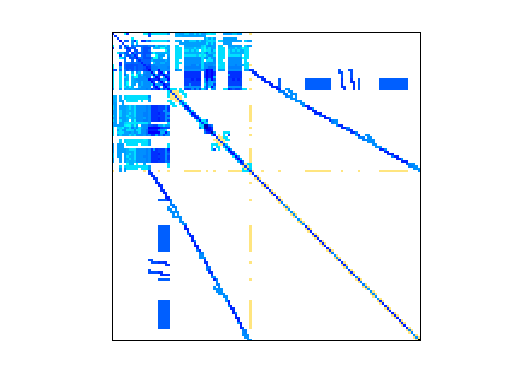
\includegraphics[width=\linewidth]{model_images/circuit5M_dc}
		\caption{circuit5M\_dc}
		\label{dat:circuit5M_dc}
	\end{subfigure}
	~
	\begin{subfigure}{0.40\linewidth}
		\centering
		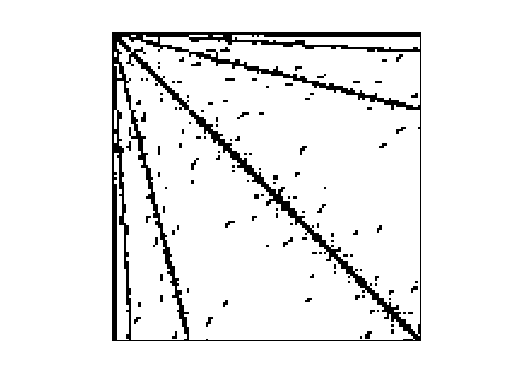
\includegraphics[width=\linewidth]{model_images/delaunay_n23}
		\caption{delaunay\_n23}
		\label{dat:delaunay_n23}
	\end{subfigure}

	\begin{subfigure}{0.40\linewidth}
		\centering
		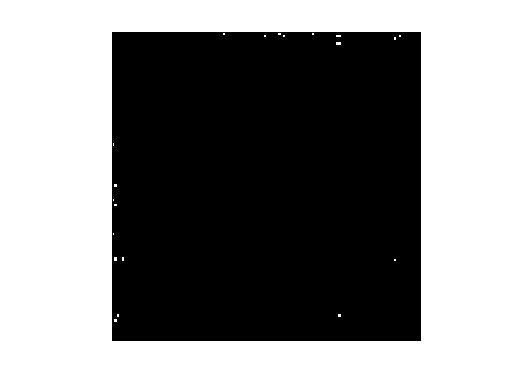
\includegraphics[width=\linewidth]{model_images/europe_osm}
		\caption{europe\_osm}
		\label{dat:europe_osm}
	\end{subfigure}
	~
	\begin{subfigure}{0.40\linewidth}
		\centering
		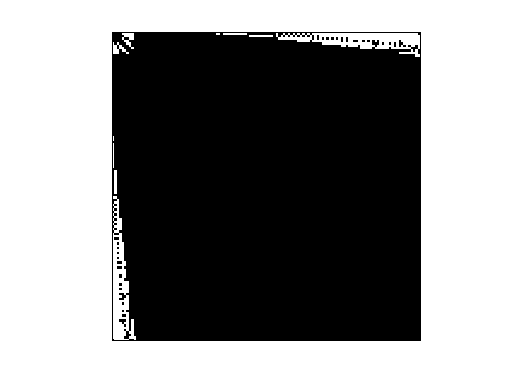
\includegraphics[width=\linewidth]{model_images/hugetrace-00000}
		\caption{hugetrace-00000}
		\label{dat:hugetrace-00000}
	\end{subfigure}

	\begin{subfigure}{0.40\linewidth}
		\centering
		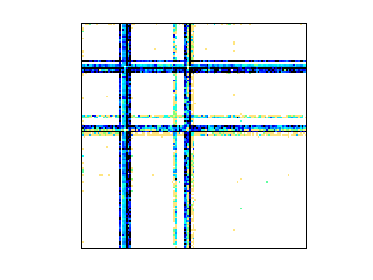
\includegraphics[width=\linewidth]{model_images/mawi_201512020330}
		\caption{mawi\_201512020330}
		\label{dat:mawi_201512020330}
	\end{subfigure}
	~
	\begin{subfigure}{0.40\linewidth}
		\centering
		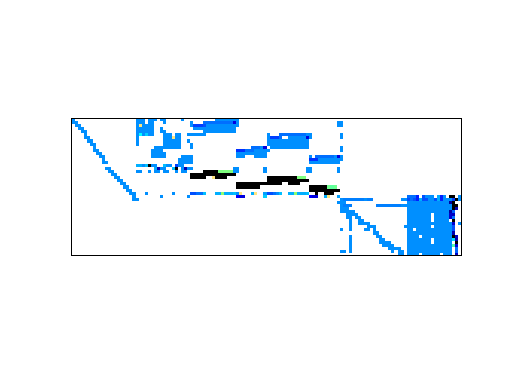
\includegraphics[width=\linewidth]{model_images/model7}
		\caption{model7}
		\label{dat:model7}
	\end{subfigure}

	\begin{subfigure}{0.40\linewidth}
		\centering
		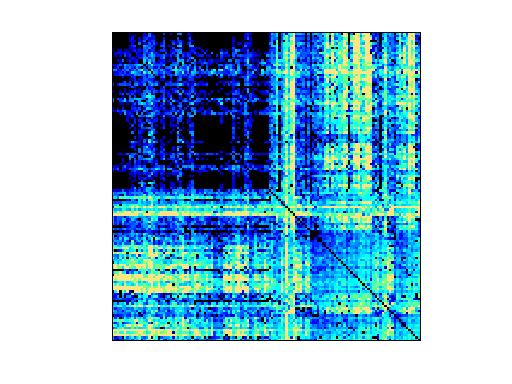
\includegraphics[width=\linewidth]{model_images/mouse_gene}
		\caption{mouse\_gene}
		\label{dat:mouse_gene}
	\end{subfigure}
	~
	\begin{subfigure}{0.40\linewidth}
		\centering
		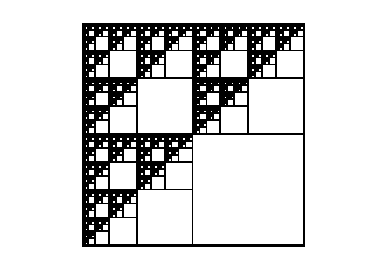
\includegraphics[width=\linewidth]{model_images/mycielskian16}
		\caption{mycielskian16}
		\label{dat:mycielskian16}
	\end{subfigure}


	\caption{Visualization of the matrices}
	\label{img:data-vis}
\end{figure}





\FloatBarrier

\section{Experimental Results}
%Present and discuss results. Include plots and tables when required (like Figure \ref{fig:enter-label}). Do not simply describe the figures; criticise the achieved results by underlining how they confirm/differ from the expected outcomes described in Section \ref{sec:methodology}.

%\noindent For the analysis include
%\begin{itemize}
%	\item Valgrind and runtime comparison between the CPU implementations
%	\item Runtime CPU vs GPU comparison looping over different matrix dimensions
%\end{itemize}
\subsection{CPU implementations}
We measured the average time (over 20 cycles with 5 warmup), and as the figure \ref{fig:time-cpu-results} shows, CSR is faster than the COO implementation in most cases. In particular, over the datasets we measured the CSR implementation is 2.48 times faster (+148\%) on average.

\begin{figure}[h!]
	\centering
	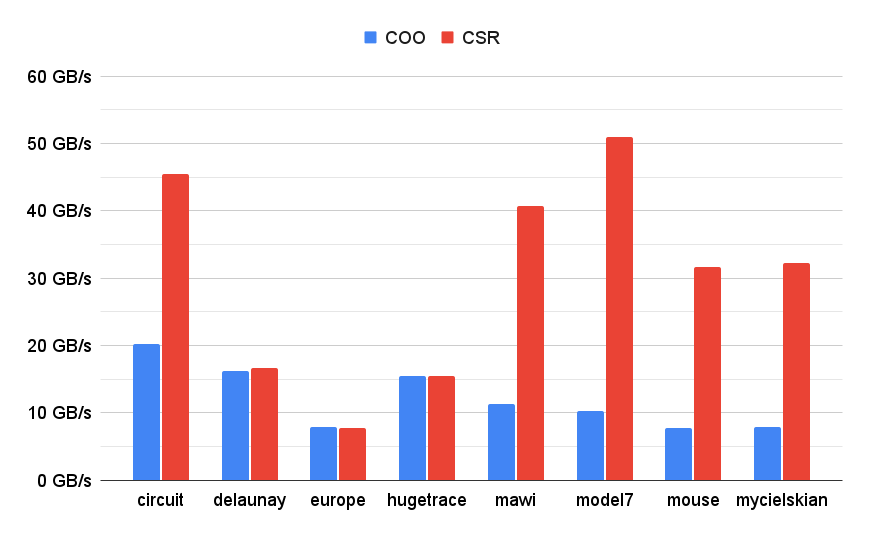
\includegraphics[width=1\linewidth]{data_images/cpu}
	\caption{CPU implementations performance over datasets}
	\label{fig:time-cpu-results}
\end{figure}

\begin{table}[h!]
	\centering
	\begin{adjustbox}{width=0.9\columnwidth}
		\begin{tabular}{lcccc}
			\toprule
			\textbf{Datasets} & \textbf{COO} & \textbf{COO} & \textbf{CSR} & \textbf{CSR} \\
			& \textbf{(ms)} & \textbf{(GBs)} & \textbf{(ms)} & \textbf{(GBs)} \\
			\midrule
			circuit & 22.71 & 20.28 & 10.12655 & 45.49 \\
			delaunay & 74.83 & 16.14 & 72.76855 & 16.60 \\
			europe & 331.19 & 7.83 & 332.649 & 7.80 \\
			hugetrace & 10.63 & 15.54 & 10.62155 & 15.54 \\
			mawi & 1015.80 & 11.34 & 282.75595 & 40.75 \\
			model7 & 0.12 & 10.27 & 0.02405 & 50.92 \\
			mouse & 88.93 & 7.82 & 21.93315 & 31.70 \\
			mycielskian & 102.37 & 32.16 & 24.88275 & 32.20 \\
		\end{tabular}
	\end{adjustbox}
	\vspace{1em}

	\caption{CPU implementations performance over datasets}
	\label{tab:time-cpu-results}
\end{table}
\FloatBarrier

In the Table \ref{tab:time-cpu-results} are also reported the bandwidth calculated from the average times, instead of the flops, that is because it is memory bound, so we care more about bandwidth. As it possible to see, CSR win in almost every case (by up to 5x in Model7), except for Hugetrace where it ties with COO and in Europe where COO is 0.38\% faster. Most of these difference can be explained by the size reduction caused by the compression ratio (can also be seen as number of rows over number of not zero entries) of the row array. The greater the compression ratio is the greater the reduction of the memory access and as such the cache misses. This can mostly explain the data, except for Mawi, which possibly doesn't follow the normal trend because of its huge size and as such is more sensible to cache misses; and Delanunay which instead only get minimal performance improvements.


\begin{figure}[h!]
	\centering
	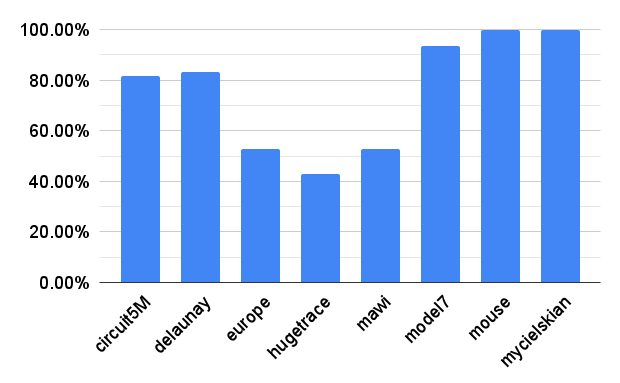
\includegraphics[width=0.7\linewidth]{data_images/csr-compression-rate}
	\caption{Compression size reduction (only considering row size)}
	\label{fig:csr-compression-rate}
\end{figure}
\FloatBarrier


To test this hypothesis we used Model7 as datasets to evaluate cache misses, and the results are the one in the Table \ref{tab:cache-results} .These values are very rough as cachegrind doesn't allow testing of a single portion of code. As such, both test were conducted in the same exact codebase with the single difference of calling COO or CSR methods (so even the conversion from COO to CSR was done in both).

This minimize the difference between the test but doesn't solve the issue of the initialization causing some misses. To reduce the impact of the initial misses, the SpMV was compute 500 times.

As expected, CSR having the rows array compressed, cause less lower reference to memory location and so it also cause slightly less cache misses.
\begin{table}[h!]
	\centering
	\begin{adjustbox}{width=\columnwidth}
		\begin{tabular}{lrrrrc}
			\toprule
			\textbf{Type} & \textbf{D Refs} & \textbf{D1 misses} & \textbf{LLd misses} & \textbf{D1 miss rate} & \textbf{LLd miss rate} \\
			\midrule
			COO & 429M & 5.35M & 13.4k & 1.2\% & 0.0\% \\
			CSR & 38M & 4.03M & 13.4k & 1.1\% & 0.0\% \\
			\bottomrule
		\end{tabular}
	\end{adjustbox}
	\vspace{1em}

	\caption{Valgrind's cachegrind tool results}
	\label{tab:cache-results}
\end{table}

Those are likely the major reason causing the COO, implementations to be slower, as all the rest is the same. In fact, as said before, here the COO is assumed to be sorted and as such the executions differ only by the memory access to the row of the two formats.

\subsection{GPU implementations}
\label{subsec:GPU}
The simple idea of a GPU Algorithm \ref{alg:COO_GPU} can be implemented in various ways. The versions tested in this paper are:
\begin{itemize}
	\item \textbf{"Kernel 1 size"}: where each thread acquires locally adjacent elements;
	\item \textbf{"Kernel threads size"}: where the distance between an element and the next that the thread acquire is the \# threads;
	\item \textbf{"Kernel warp size"}: where the distance between an element and the next that the thread acquire is the size of a warp;
	\item \textbf{"Kernel block size"}: where the distance between an element and the next that the thread acquire is the size of a block;
\end{itemize}

It was, then, tested the performance of them, with respect to the number of thread per block and the number of blocks. As expected the first kernel is the worst one and warp size and block size are in the first place, while perform around the same. This is because of the fact that warp share cache and as such threads in same thread should access close position. The reason for "Kernel threads size" to be about half the performance of the warp one it is possibly connected to the fact that each thread need to access location that are pretty far apart, increasing cache misses.

\begin{figure}[h!]
	\centering
	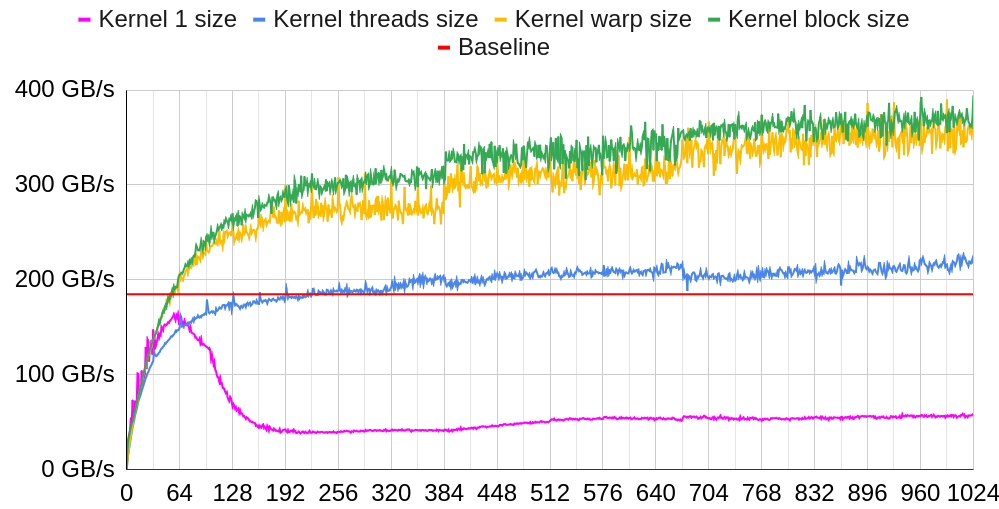
\includegraphics[width=1\linewidth]{data_images/Gb_for_size_block_2}
	\caption{Throughput over block size of the various kernels}
	\label{fig:gbforsizeblock2}
\end{figure}


\begin{figure}[h!]
	\centering
	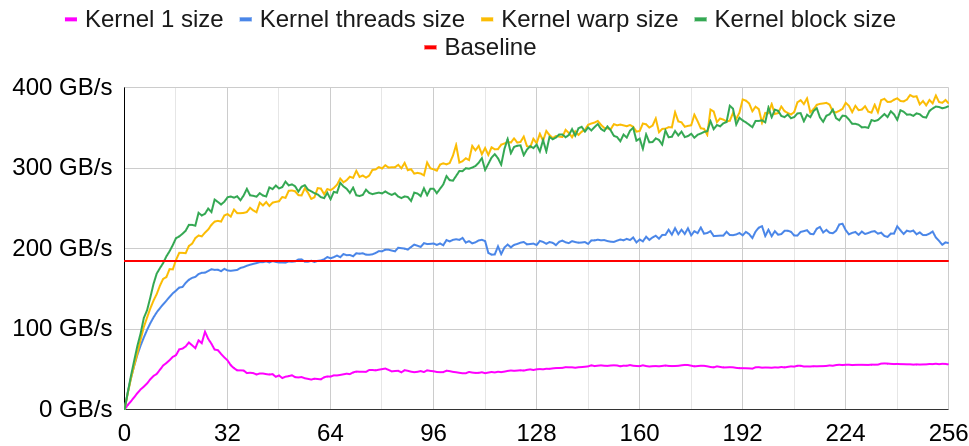
\includegraphics[width=1\linewidth]{data_images/Gb_for_size_grid_2}
	\caption{Throughput over blocks number of the various kernels}
	\label{fig:gbforsizegrid2}
\end{figure}

\FloatBarrier
Also as expected the two graph look very alike.

The kernels were then benchmarked with all the datasets, using the best parameter, those being 1024 threads for blocks and with 256 blocks.

\begin{figure}[h!]
	\centering
	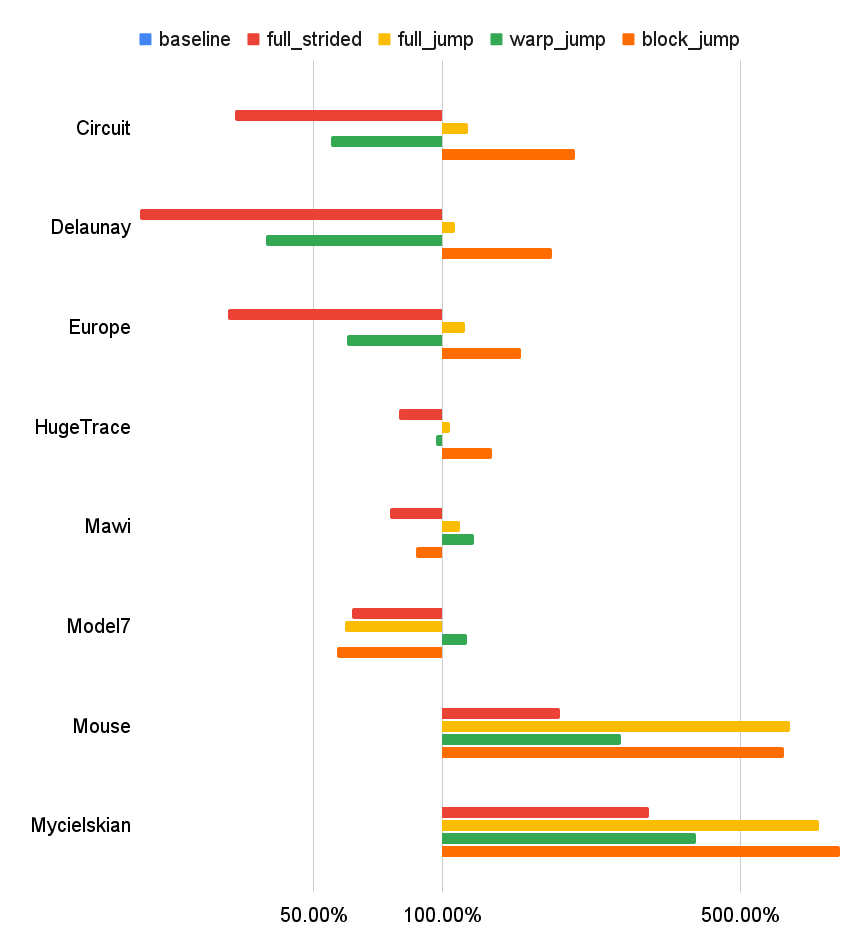
\includegraphics[width=0.9\linewidth]{data_images/perf_gpu}
	\caption{Performance of the kernels based on dataset with respect to baseline}
	\label{fig:perf-gpu}
\end{figure}

And reported in the following table are the best kernel version and their respective improvements.

\begin{table}[h!]
	\centering
	\begin{adjustbox}{width=0.9\columnwidth}
		\begin{tabular}{lccc}
			\toprule
			\textbf{Datasets} & \textbf{Baseline } &\textbf{Best } & \textbf{Improvement }\\
			& (GBs) & \textbf{kernel} & \textbf{over baseline} \\
			\midrule
			circuit &177.183& block\_jump & 1.15  \\
			delaunay &204.727 & block\_jump & 1.07 \\
			europe & 99.8868& block\_jump & 1.13  \\
			hugetrace &72.1631 & block\_jump & 1.04  \\
			mawi &23.71207614 & warp\_jump & 1.45  \\
			model7 &2.34113 & warp\_jump & 1.14 \\
			mouse & 53.7371&  block\_jump & 6.54  \\
			mycielskian& 36.9665& block\_size & 7.65 \\
		\end{tabular}
	\end{adjustbox}

	\caption{Results in table format}
	\label{tab:gpu-results}
\end{table}

\FloatBarrier
As it was expected, the worst performance come from the smallest dataset. The cause of this, is that GPU are optimized for throughput and so they have higher latency. So with smaller size datasets the latency become the limiting factor. For this reason we are less interested in them, as the comparison between the various kernel become less important, as most of the spent time is on the overhead (eg. creating a kernel).



Finally we can note, ignoring Model7, the "Kernel block size" has the most reliable performance as expected; while "Kernel warp size" has better performance only on Mawi by some margin. This is possibly related to the huge size of the matrix, but because of that, it is not possible to profile it.

In figure \ref{fig:cpu-vs-gpu}, as expected, the GPU implementations are generally much faster. On average the GPU implementation is 17.4x faster than the COO implementation and 7x faster then the CSR implementation. Model7, again show that GPU are not always the solution and for such a small matrix, the GPU overhead and the slower single core performance impact so much that the GPU version is less than half the speed of the CPU CSR; for this reason we will be ignoring it from now on. The only other outlier is mawi which contains row so dense that having them compressed have a big impact on performance as shown by the fact the CSR implementation can beat it even though it is run on CPU. But with the coming optimization the GPU version will be able to be faster than CSR version.

\begin{figure}[h!]
	\centering
	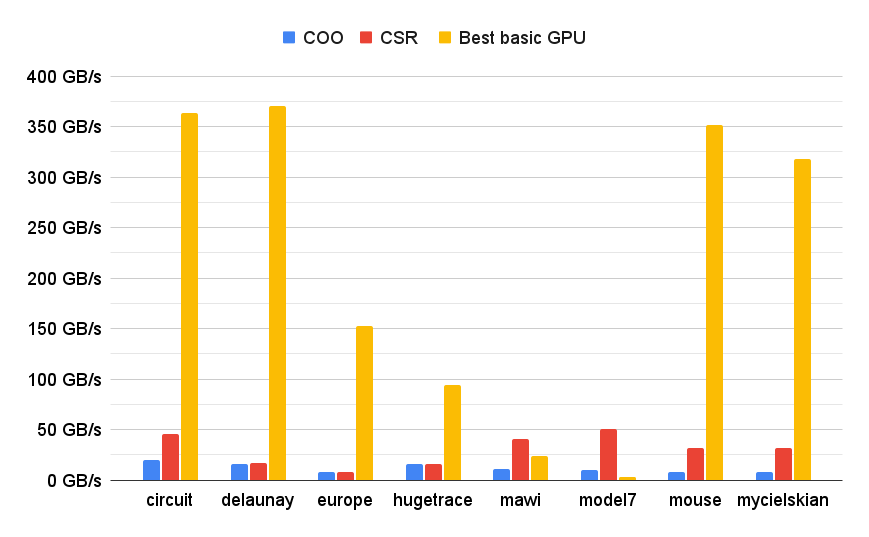
\includegraphics[width=0.9\linewidth]{data_images/cpu-vs-gpu}
	\caption{Comparison with CPU. COO CPU is baseline.}
	\label{fig:cpu-vs-gpu}
\end{figure}
\FloatBarrier

\subsection{Prefix sum}
In the figure \ref{fig:prefix-sum}, we compare multiple kernel implementation of the prefix sum. Some of them are 32, while other are 1024 in the sense whether or not the prefix sum is performed over WARP or BLOCK size. Also there are the various optimization presented in the previous chapter, such as using warp primitive and using prefix sum only over the same row to remove extra write to result vector.

\begin{figure}[h!]
	\centering
	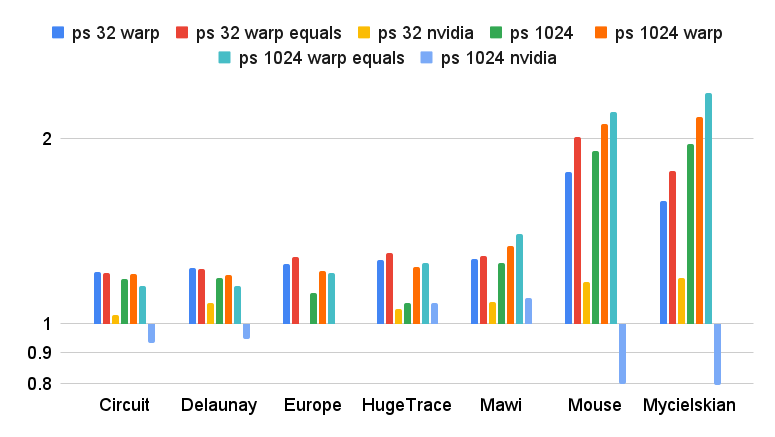
\includegraphics[width=1\linewidth]{data_images/prefix-sum}
	\caption{Various prefix sum over "ps 32" as baseline}
	\label{fig:prefix-sum}
\end{figure}
\FloatBarrier



As the graph show, the best performing overall both for the 32 and the 1024 case are the one that use warp primitive because as the NCU should it reduce the number of time the threads are stalled waiting for memory. That is the case in the first algorithm, because each thread is trying to access the shared memory causing it bank conflict.

Finally, we want to make note of the result of the kernel from the NVIDIA book, it should be a work efficient prefix sum without bank conflict, but it under-performs here. We were able to test that, this is only the case on A30 of `edu01`, while the performs much better on the L40s of `edu02`, possibly because of the much higher peak arithmetic performance, but this is outside the scope of this paper.

We finally implemented a kernel that put together the "Kernel prefix Jump" of the previous section and the "ps 32 warp equals". It was also tested the loop unroll feature of CUDA as final optimization.

\begin{figure}[h!]
	\centering
	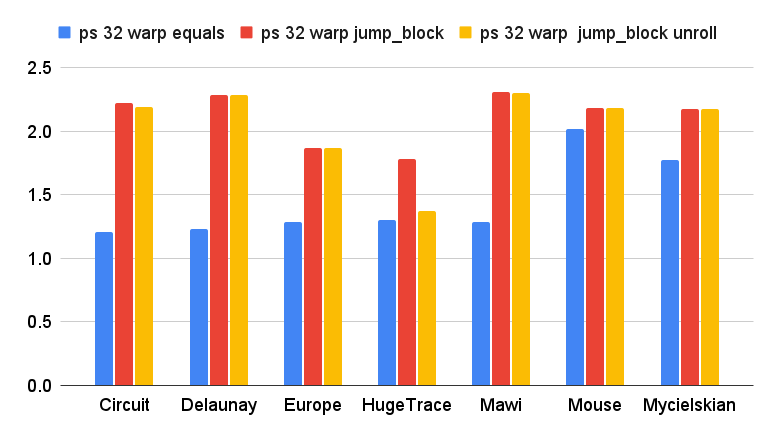
\includegraphics[width=1\linewidth]{data_images/last-prefix}
	\caption{Performance using also block jump and unroll}
	\label{fig:last-prefix}
\end{figure}

While the increase in performance for the block jump is obtained, that is not the case for the loop unroll. CUDA already loop unroll based on heuristic and increasing how much it is unroll may be counterproductive, increasing the number of cache misses for the code.


\section{Conclusions}
In conclusion, we were able to create a kernel that is up to tens of times faster than baseline (10x for mawi, 20x for Mouse and 30x for Mycielskian). This brings the totals result to the one in figure \ref{fig:overall} .



\begin{figure}[hbt!]
	\centering
	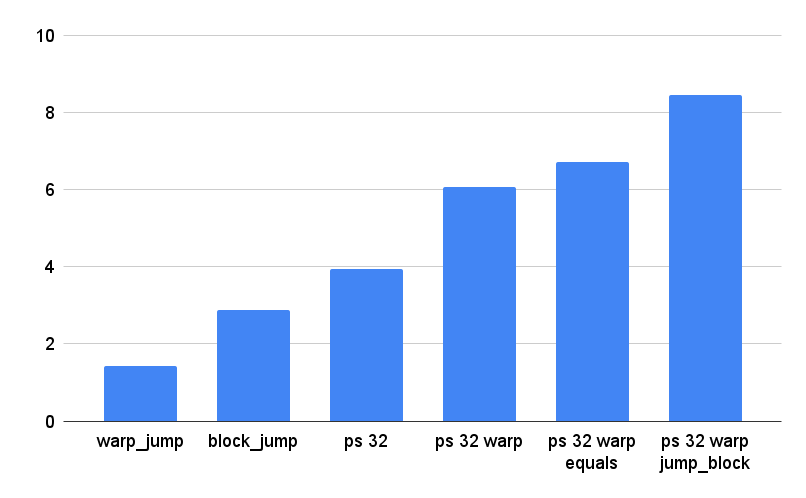
\includegraphics[width=1\linewidth]{data_images/overall}
	\caption{Average of improvements over baseline}
	\label{fig:overall}
\end{figure}

These results are strongly skewed by the row dense matrices. But, as it is possible to see in the table \ref{tab:best_kernels}, ignoring the prefix sum 1024 versions which are best for very dense row matrix, all of the rest of the datasets have the best performance on prefix sum 32 warp jump\_block (at most the unroll version).

\begin{table}[h!]
	\centering
	\begin{adjustbox}{width=0.9\columnwidth}
		\begin{tabular}{lcc}
			\toprule
			\textbf{Datasets} & \textbf{Best kernel} & \textbf{GBs} \\
			\midrule
	        Circuit & ps 32 warp jump\_block & 363.2216063 \\
			Delaunay & ps 32 warp  jump\_block unroll & 412.0683638 \\
			Europe & ps 32 warp  jump\_block unroll & 153.8266709 \\
			HugeTrace & ps 32 warp jump\_block & 95.11313069 \\
			Mawi & ps 32 warp  jump\_block unroll & 186.3647494 \\
			Mouse & ps 1024 warp equals & 1098.117639 \\
			Mycielskian & ps 1024 warp equals & 1219.720757 \\
		\end{tabular}
	\end{adjustbox}

	\caption{Results in table format}
	\label{tab:best_kernels}
\end{table}

So, we can conclude that the prefix warp version is best among most of the one proposed in here in all scenarios. The only thing that remain to evaluate is whether or not to use the 1024 version. But as said before the 1024 version is best when the matrix is very row dense. We can easily check than in O(n), but is still need to be tested the feasibility of a O(n) before the kernel execution.

Finally, while the relative time ratio are accurate, as it is possible to see from the previous table, the bandwidth goes over the maximum for the A30. That is the case, because the actual arithmetic intensity increased, as the number of load and write to the resulting vector decreased.

\subsection{Limitations}
Because of multiple node downtime, task with priority, and profiler stopping working and throwing down the entire node, it was not possible to obtain reliable and comparable data using NCU. Because of that, it was only used to gain some insight but could not be used to demonstrate the reason behind the optimization gains.


\end{document}

